\documentclass[a4paper,11pt,fleqn]{article}%fleqn pour aligner les equations à gauche
\usepackage{../../Styles/Cours}

\newcommand{\chnum}{Chapitre 18}
\newcommand{\chtitle}{Interférences lumineuses}
\newcommand{\dtype}{TP}

  
\begin{document}
\maketitle

\textbf{Rappels du TP précédent :}\\

1. Nommer puis décrire le phénomène observé lorsqu'un faisceau laser rencontre un obstacle de petit diamètre (fil ou fente).\\
\noindent
\fbox{\begin{minipage}{\linewidth}
\vspace{3cm}
\hspace{3cm}
\end{minipage}}

\begin{minipage}{.35\linewidth}
2. Annoter le schéma ci-contre.
\end{minipage}
\begin{minipage}{.6\linewidth}
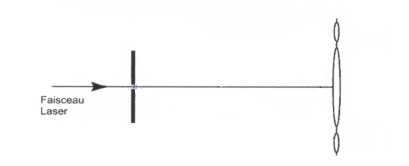
\includegraphics[scale=.75]{Ressources/TSPE_C9_AE3_Fig4.png}
\end{minipage}



On remplace dans le montage précédent, le fil par une diapositive noire comptant trois doubles fentes d'écartement $b$ différents. L'une de ces doubles fentes est placée devant le faisceau laser.\\

3. Proposer un schéma annoté du montage.$\rightarrow$
\noindent
\fbox{\begin{minipage}{.45\linewidth}
\vspace{3cm}
\hspace{3cm}
\end{minipage}}


4. Réaliser le montage.\\

5. Décrire la figure observée sur l'écran.\\
\noindent
\fbox{\begin{minipage}{\linewidth}
\vspace{2cm}
\hspace{3cm}
\end{minipage}}

\vspace{.5cm}
On appelle interfrange $i$ la distance séparant les milieux de deux franges brillantes consécutives sur l'écran.\\

6. Comment varie $i$ lorsque $b$ diminue ? Justifier votre réponse en se basant sur les mesures expérimentales.\\
\noindent
\fbox{\begin{minipage}{\linewidth}
\vspace{2.5cm}
\hspace{3cm}
\end{minipage}}

\vspace{.5cm}

\newpage
7. La valeur de l'interfrange $i$ dépend-t-elle de la distance entre le laser et l'écran ou de la distance entre les fentes et l'écran ? Proposer un protocole rapide pour vérifier cette réponse.\\
\noindent
\fbox{\begin{minipage}{\linewidth}
\vspace{3cm}
\hspace{3cm}
\end{minipage}}
\vspace{.5cm}
8. Mettre en \oe uvre le protocole et compléter les tableaux suivants :
\begin{center}
\begin{tabular}{|>{\centering}m{1.7cm}|>{\centering}m{1.7cm}|>{\centering}m{1.7cm}|>{\centering\arraybackslash}m{1.7cm}|}
    \hline $D$ en m &   &  & \rule[1cm]{0cm}{0cm}\\
    \hline $i$ en mm & & & \rule[1cm]{0cm}{0cm}\\ \hline
\end{tabular}
\begin{tabular}{|>{\centering}m{1.7cm}|>{\centering}m{1.7cm}|>{\centering}m{1.7cm}|>{\centering\arraybackslash}m{1.7cm}|}
    \hline $D$ en m &   &  & \rule[1cm]{0cm}{0cm}\\
    \hline $i$ en mm & & & \rule[1cm]{0cm}{0cm}\\ \hline
\end{tabular}
\end{center}

On ajuste la distance entre les fentes et l'écran à $D$ = \num{1,50} \unit{\meter}.\\

9. Mesurer pour plusieurs valeurs d'écartement $b$, la valeur de l'interfrange $i$ et compléter le tableau suivant.
\begin{center}
\begin{tabular}{|>{\centering}m{2cm}|>{\centering}m{2cm}|>{\centering}m{2cm}|>{\centering\arraybackslash}m{2cm}|}
    \hline $b$ en mm &   &  & \\
    \hline $i$ en mm & & & \rule[1cm]{0cm}{0cm} \\ \hline
\end{tabular}
\end{center}

10. Sur un tableur de votre choix, tracer la courbe $i = f(\dfrac{1}{b}$).\\

11. Déduire de la question précédente que l'interfrange peut s'exprimer comme une fonction de $1/b$.\\
\noindent
\fbox{\begin{minipage}{\linewidth}
\vspace{2.5cm}
\hspace{3cm}
\end{minipage}}

\vspace{.5cm}
12. À partir de la courbe $i = f(\dfrac{1}{b}$), calculer la longueur d'onde $\lambda$ du laser et comparer la valeur expérimentale à celle du fabricant en calculant l'écart relatif entre les deux valeurs.\\
\noindent
\fbox{\begin{minipage}{\linewidth}
\vspace{2.5cm}
\hspace{3cm}
\end{minipage}}

\vspace{.5cm}
13. Calculer la valeur d'incertitude relative à la détermination de $\lambda$, notée $u(\lambda)$.\\
Rappel : $\dfrac{u(\lambda)}{\lambda} = \sqrt{\left(\dfrac{u(D)}{D}\right)^2 + \left(\dfrac{u(b)}{b}\right)^2 + \left(\dfrac{u(i)}{i}\right)^2}$\\
\noindent
\fbox{\begin{minipage}{\linewidth}
\vspace{3cm}
\hspace{3cm}
\end{minipage}}

\vspace{.5cm}
\end{document}